\documentclass{beamer}
\usepackage{tikz}
\usepackage{CJKutf8}
\usepackage{graphicx}
\begin{document}
\begin{CJK}{UTF8}{gbsn}
\newtheorem{definition9.1.1}{定义9.1.1}
\newtheorem{definition9.1.2}{定义9.1.2}
\newtheorem{theorem9.1.1}{定理9.1.1(欧拉公式)}
\newtheorem{corollary9.1.1}{推论9.1.1}
\newtheorem{corollary9.1.2}{推论9.1.2}
\newtheorem{corollary9.1.3}{推论9.1.3}
\newtheorem{corollary9.1.4}{推论9.1.4}
\newtheorem{corollary9.1.5}{推论9.1.5}
\newtheorem{corollary9.1.6}{推论9.1.6}
\newtheorem{theorem9.2.1}{定理9.2.1}
\newtheorem{definition9.3.1}{定义9.3.1}
\newtheorem{definition9.3.2}{定义9.3.2}
\newtheorem{definition9.3.3}{定义9.3.3}
\newtheorem{definition9.3.4}{定义9.3.4}
\newtheorem{theorem9.3.1}{定理9.3.1}
\newtheorem{theorem9.3.2}{定理9.3.2}
\newtheorem{definition9.4.1}{定义9.4.1}
\newtheorem{definition9.4.2}{定义9.4.2}
\newtheorem{theorem9.4.1}{定理9.4.1}
\newtheorem{theorem9.4.2}{定理9.4.2}
\newtheorem{theorem9.4.3}{定理9.4.3}
\newtheorem{theorem9.4.4}{定理9.4.4}
\newtheorem{theorem9.4.5}{定理9.4.5}
\newtheorem{theorem9.4.6}{定理9.4.6}
\newtheorem{exercise1}{习题1}
\newtheorem{exercise2}{习题2}
\newtheorem{exercise3}{习题3}
\newtheorem{exercise4}{习题4}
\newtheorem{exercise5}{习题5}
\newtheorem{Exercise}{习题}

\date{}
\author{陈建文}

\title{第九章 平面图和图的着色}
\begin{frame}
  \titlepage
  
\end{frame}
\begin{frame}
  \frametitle{第九章 平面图和图的着色}
\end{frame}

\begin{frame}
  \frametitle{第九章 平面图和图的着色}
  \begin{enumerate}
  \item 平面图\\
\pause
在印刷电路的布线中,人们感兴趣的是要知道一个特定的电网络是否可以嵌入平面上。
\pause
\item 图的着色\\
\pause
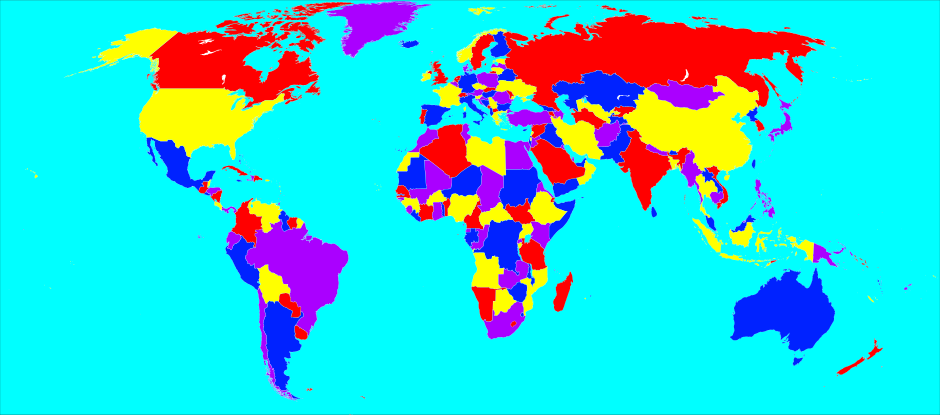
\includegraphics[width=5cm,height=3cm]{Worldmap}
  \end{enumerate}
\end{frame}

% \begin{frame}
%   \frametitle{9.1 平面图及其欧拉公式}
%   \begin{definition9.1.1}
%     图$G$称为被嵌入平(曲)面$S$内,如果$G$的图解已画在$S$上,而且任何两条边均不相交(除可能在端点相交外)。
% 已嵌入平面内的图称平面图。如果一个图可以嵌入平面,则称此图是可平面的。
%   \end{definition9.1.1}
% 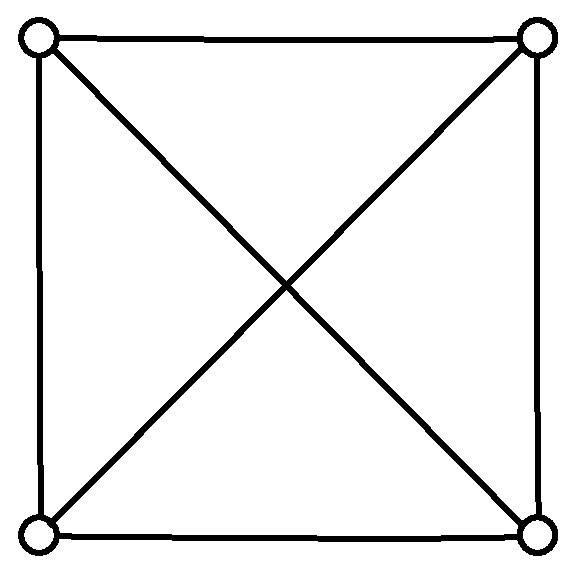
\includegraphics[width=4cm,height=3cm]{k4}
% \end{frame}

\begin{frame}
  \frametitle{9.1 平面图及其欧拉公式}
\pause
  \begin{definition9.1.1}
    图$G$称为被嵌入平(曲)面$S$内,如果$G$的图解已画在$S$上,而且任何两条边均不相交(除可能在端点相交外)。
已嵌入平面内的图称\alert{平面图}。如果一个图可以嵌入平面,则称此图是\alert{可平面}的。

\end{definition9.1.1}
%   \begin{minipage}{0.45\linewidth}
% 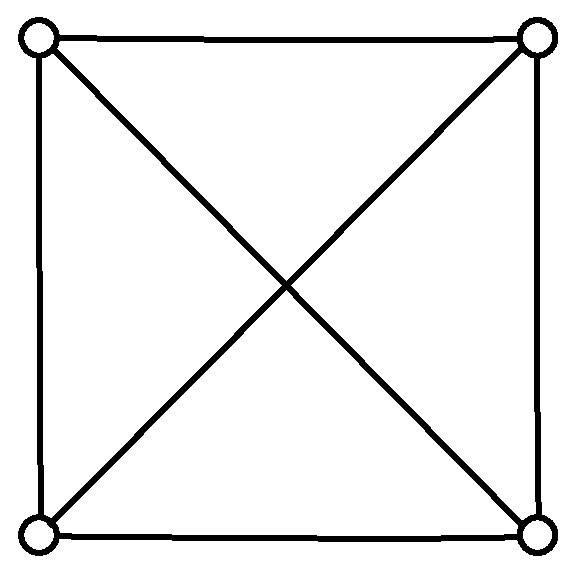
\includegraphics[width=4cm,height=3cm]{k4}    
%   \end{minipage}
%   \begin{minipage}{0.45\linewidth}
%     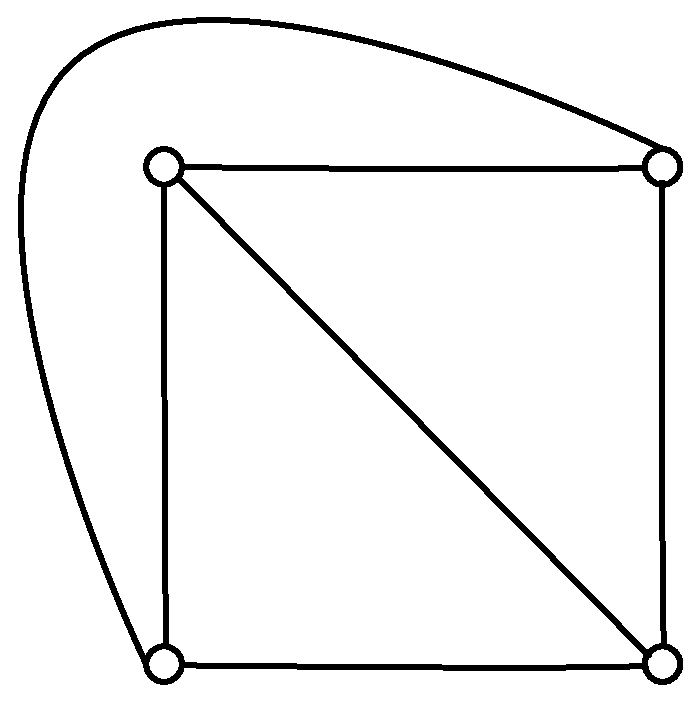
\includegraphics[width=4cm,height=3cm]{k4planar}
%   \end{minipage}
\end{frame}

\begin{frame}
  \frametitle{9.1 平面图及其欧拉公式}
%   \begin{definition9.1.1}
%     图$G$称为被嵌入平(曲)面$S$内,如果$G$的图解已画在$S$上,而且任何两条边均不相交(除可能在端点相交外)。
% 已嵌入平面内的图称平面图。如果一个图可以嵌入平面,则称此图是可平面的。
%   \end{definition9.1.1}
  \begin{minipage}{0.45\linewidth}
\includegraphics[width=4cm,height=3cm]{k5}    
  \end{minipage}
\pause
  \begin{minipage}{0.45\linewidth}
    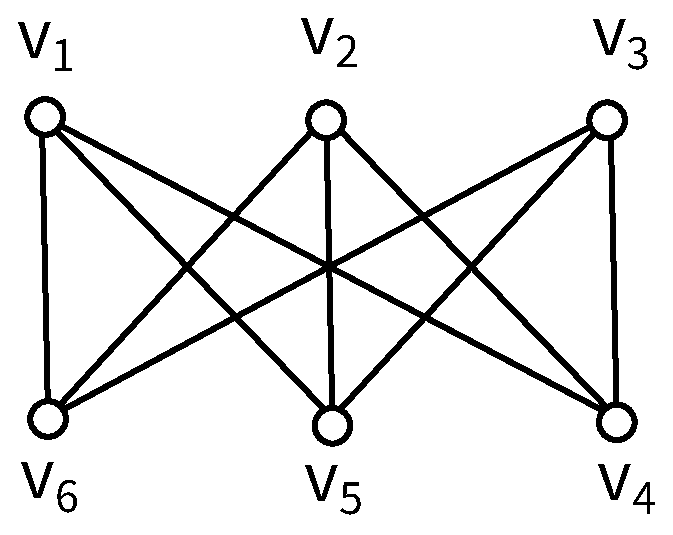
\includegraphics[width=4cm,height=3cm]{k33}
  \end{minipage}
\pause
  \begin{thebibliography}{99}
  \bibitem[Hopcroft, 1974]{Hopcropt1974}J. Hopcroft and R. Tarjan.
\newblock Efficient planarity testing.
\newblock Journal of the Association for Computing Machinery, 21(4):549-568, 1974.
  \end{thebibliography}
\pause
  \begin{thebibliography}{99}
  \bibitem[Boyer, 2004]{Boyer2004}J. Boyer and W. Myrvold.
\newblock On the Cutting Edge: Simplified O(n) Planarity by Edge Addition.
\newblock Journal of Grah algorithms and Applications, 8(3):241-273, 2004.
  \end{thebibliography}
\end{frame}
\begin{frame}
  \frametitle{9.1 平面图及其欧拉公式}
  \begin{definition9.1.2}
    平面图$G$把平面分成了若干个区域,这些区域都是连通的,称之为$G$的\alert{面},其中无界的那个连通区域称为$G$的\alert{外部面},其余的连通区域称为$G$的\alert{内部面}。
    
\includegraphics[width=4cm,height=3cm]{face}
  \end{definition9.1.2}
\end{frame}
\begin{frame}
  \frametitle{9.1 平面图及其欧拉公式}
  \begin{theorem9.1.1}
    如果有$p$个顶点$q$条边的平面连通图$G$有$f$个面,则
      $p - q + f = 2$
  \end{theorem9.1.1}
\vspace{1cm}
\centering
    \includegraphics[width=4cm,height=3cm]{euler}
\end{frame}

\begin{frame}
  \frametitle{9.1 平面图及其欧拉公式}
  \begin{theorem9.1.1}
    如果有$p$个顶点$q$条边的平面连通图$G$有$f$个面,则
      $p - q + f = 2$
  \end{theorem9.1.1}
\vspace{1cm}
\centering
    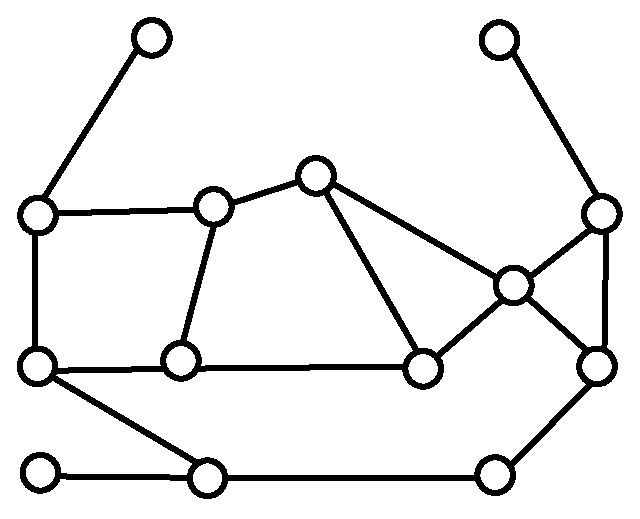
\includegraphics[width=4cm,height=3cm]{euler1}
\end{frame}
\begin{frame}
  \frametitle{9.1 平面图及其欧拉公式}
  \begin{theorem9.1.1}
    如果有$p$个顶点$q$条边的平面连通图$G$有$f$个面,则
      $p - q + f = 2$
  \end{theorem9.1.1}
\vspace{1cm}
\centering
    \includegraphics[width=4cm,height=3cm]{euler2}
\end{frame}
\begin{frame}
  \frametitle{9.1 平面图及其欧拉公式}
  \begin{theorem9.1.1}
    如果有$p$个顶点$q$条边的平面连通图$G$有$f$个面,则
      $p - q + f = 2$
  \end{theorem9.1.1}
\vspace{1cm}
\centering
    \includegraphics[width=4cm,height=3cm]{euler3}
\end{frame}
\begin{frame}
  \frametitle{9.1 平面图及其欧拉公式}
  \begin{theorem9.1.1}
    如果有$p$个顶点$q$条边的平面连通图$G$有$f$个面,则
      $p - q + f = 2$
  \end{theorem9.1.1}
\vspace{1cm}
\centering
    \includegraphics[width=4cm,height=3cm]{euler4}
\end{frame}
\begin{frame}
  \frametitle{9.1 平面图及其欧拉公式}
  \begin{theorem9.1.1}
    如果有$p$个顶点$q$条边的平面连通图$G$有$f$个面,则
      $p - q + f = 2$
  \end{theorem9.1.1}
\vspace{1cm}
\centering
    \includegraphics[width=4cm,height=3cm]{euler5}
\end{frame}

\begin{frame}
  \frametitle{9.1 平面图及其欧拉公式}
  \begin{theorem9.1.1}
    如果有$p$个顶点$q$条边的平面连通图$G$有$f$个面,则
      $p - q + f = 2$
  \end{theorem9.1.1}
\vspace{1cm}
\centering
    \includegraphics[width=4cm,height=3cm]{euler6}
\end{frame}

\begin{frame}
  \frametitle{9.1 平面图及其欧拉公式}
  \begin{theorem9.1.1}
    如果有$p$个顶点$q$条边的平面连通图$G$有$f$个面,则
      $p - q + f = 2$
  \end{theorem9.1.1}
\vspace{1cm}
\centering
    \includegraphics[width=4cm,height=3cm]{euler}
\end{frame}

\begin{frame}
  \frametitle{9.1 平面图及其欧拉公式}
  \begin{corollary9.1.1}
    若平面图$G$有$p$个顶点$q$条边且每个面都是由长为$n$的圈围成的,则
    \begin{equation*}
      q = n(p-2)/(n-2)
    \end{equation*}
  \end{corollary9.1.1}
\end{frame}
\begin{frame}
  \frametitle{9.1 平面图及其欧拉公式}
一个\alert{最大可平面图}是一个可平面图,对此可平面图中不能再加入边而不破坏可平面性。
  \begin{corollary9.1.2}
    设$G$是一个有$p$个顶点$q$条边的最大可平面图,$p \geq 3$,则$G$的每个面都是三角形,而且$q=3p-6$。
  \end{corollary9.1.2}
\end{frame}
\begin{frame}
  \frametitle{9.1 平面图及其欧拉公式}
  \begin{corollary9.1.3}
    设$G$是一个$(p,q)$可平面连通图,而且$G$的每个面都是一个长为$4$的圈围成的,则$q=2p-4$。
  \end{corollary9.1.3}
\end{frame}
\begin{frame}
  \frametitle{9.1 平面图及其欧拉公式}
  \begin{corollary9.1.4}
    若$G$是一个有$p$个顶点$q$条边的可平面图,$p\geq 3$,则$q \leq 3p - 6$;进一步,若$G$中没有三角形,则$q \leq 2p -4$。
  \end{corollary9.1.4}
  
      \pause
      \centering
    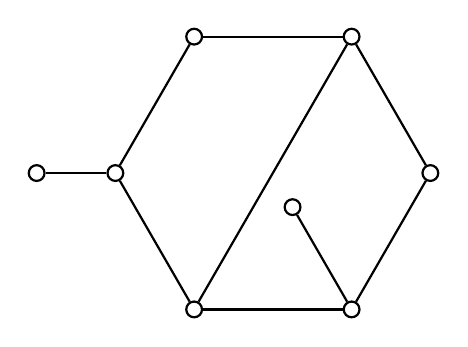
\begin{tikzpicture}[auto,
    specification/.style ={circle, draw, thick, inner sep = 0pt, minimum size=2mm}]
   \node[specification] (A)  at (0:2cm)  {};
   \node[specification] (B)  at (60:2cm)  {};
   \node[specification] (C)  at (120:2cm)  {};
   \node[specification] (D) at (180:2cm)  {};
   \node[specification] (E)  at (240:2cm)  {};   
   \node[specification] (F)  at (300:2cm)  {};   
   \node[specification] (G)  at (300:0.5cm)  {};
   \node[specification] (H)  at (180:3cm)  {};
   
   
   \draw[thick] (A) to  (B);
   \draw[thick] (B) to  (C);
   \draw[thick] (C) to  (D);
   \draw[thick] (D) to  (E);
   \draw[thick] (E) to  (F);
   \draw[thick] (F) to  (A);
   \draw[thick] (B) to  (E);
   \draw[thick] (F) to  (G);
   \draw[thick] (D) to  (H);   
 \end{tikzpicture}

\end{frame}
\begin{frame}
  \frametitle{9.1 平面图及其欧拉公式}
  \begin{corollary9.1.5}
    $K_5$和$K_{3,3}$都不是可平面图。
  \end{corollary9.1.5}
\vspace{1cm}
  \begin{minipage}{0.45\linewidth}
\includegraphics[width=4cm,height=3cm]{k5}    
  \end{minipage}
  \begin{minipage}{0.45\linewidth}
    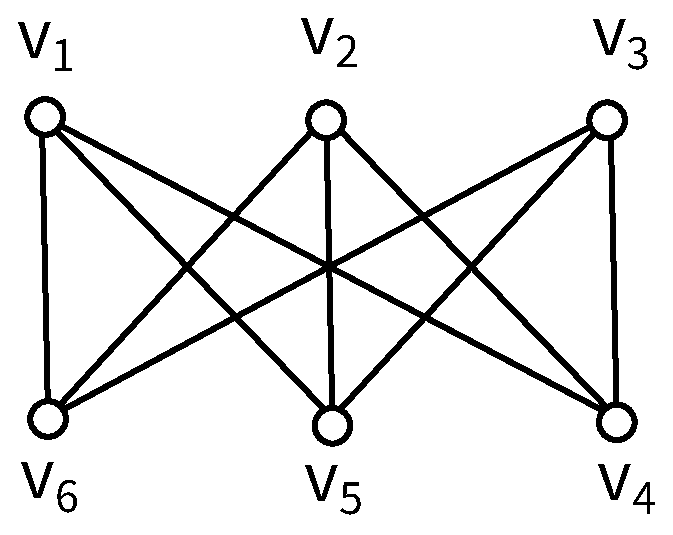
\includegraphics[width=4cm,height=3cm]{k33}
  \end{minipage}
\end{frame}
\begin{frame}
  \frametitle{9.1 平面图及其欧拉公式}
  \begin{corollary9.1.6}
    每个可平面图$G$中顶点度的最小值不超过5,即$\delta (G) \leq 5$。
  \end{corollary9.1.6}
\end{frame}
\begin{frame}
  \frametitle{9.1 平面图及其欧拉公式}
  \begin{exercise1}
    设$G$是一个有$p$个顶点的平面图,$p \geq 4$。证明:$G$中有4个度不超过5的顶点。
  \end{exercise1}
\end{frame}
\begin{frame}
  \frametitle{9.1 平面图及其欧拉公式}
  \begin{exercise2}
    设$G$是一个有$k$个支的平面图。若$G$的顶点数、边数、面数分别为$p$,$q$和$f$,试证:
    \begin{equation*}
      p - q + f = k + 1
    \end{equation*}
  \end{exercise2}
\end{frame}

\begin{frame}
  \frametitle{9.1 平面图及其欧拉公式}
  \begin{exercise3}
    若$G$是顶点数$p > 11$的平面图,试证$G^c$不是平面图。
  \end{exercise3}
\end{frame}
\begin{frame}
  \frametitle{9.1 平面图及其欧拉公式}
  \begin{exercise4}
    设$S = \{x_1, x_2, \ldots, x_n\}$ 是平面上$n$个顶点的集合,$n \geq 3$, 其中任两个顶点的距离至少是1。证明:$S$中至多有$3n-6$对顶点,其距离为1。
  \end{exercise4}
\end{frame}
\begin{frame}
  \frametitle{9.1 平面图及其欧拉公式}
  \begin{exercise5}
    证明:不存在7条棱的凸多面体。
  \end{exercise5}
\end{frame}

\begin{frame}
  \frametitle{9.2 非哈密顿平面图}
  \begin{theorem9.2.1}
    设$G=(V,E)$是一个$(p,q)$平面哈密顿图,$C$是$G$的哈密顿圈。
    令$f_i$为$C$的内部由$i$条边围成的面的个数,$g_i$为$C$的外部$i$条边围成的面的个数,则
    \begin{align}
      &1 \cdot f_3 + 2 \cdot f_4 + 3 \cdot f_5 + \cdots = \sum_{i=3}^p(i-2)f_i = p - 2;\\
      &1 \cdot g_3 + 2 \cdot g_4 + 3 \cdot g_5 + \cdots = \sum_{i=3}^p(i-2)g_i = p - 2;\\
      &1 \cdot (f_3 - g_3) + 2 \cdot (f_4 - g_4) + 3 \cdot (f_5 - g_5) + \cdots = \sum_{i=3}^p(i-2)(f_i - g_i) = 0
    \end{align}
  \end{theorem9.2.1}
\end{frame}

\begin{frame}
  \frametitle{9.2 非哈密顿平面图}
  \centering
  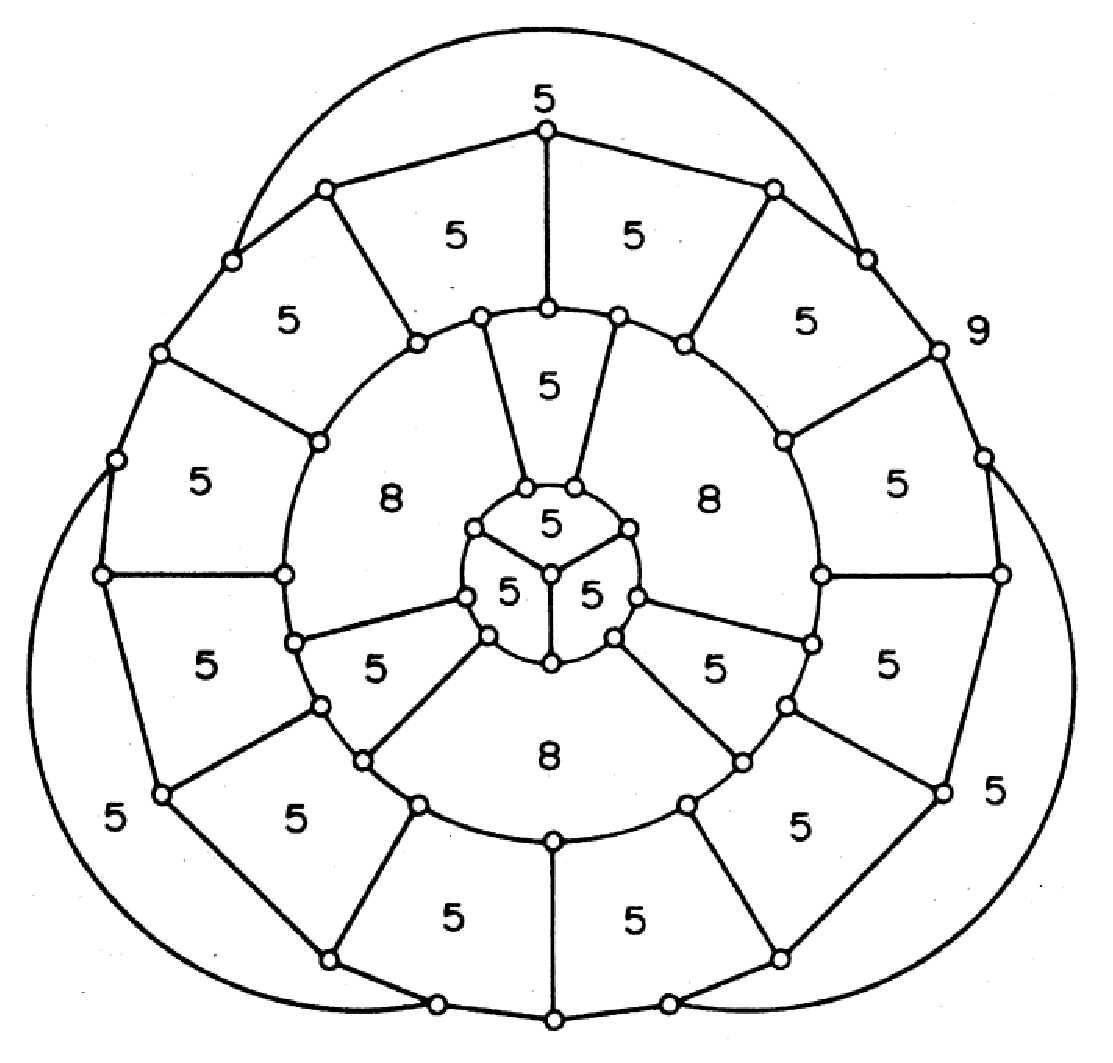
\includegraphics[width=7cm, height=6cm]{grinberg}
\end{frame}

\begin{frame}
  \frametitle{9.2 非哈密顿平面图}
  \centering
  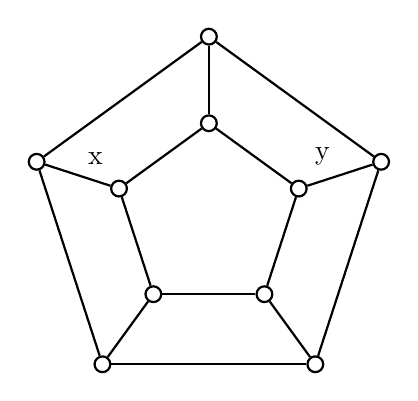
\begin{tikzpicture}[auto,
    specification/.style ={circle, draw, thick, inner sep = 0pt, minimum size=2mm}]
   \node[specification] (A)  at (18:2.3cm)  {};
   \node[specification] (B)  at (90:2.3cm)  {};
   \node[specification] (C)  at (162:2.3cm)  {};
   \node[specification] (D) at (234:2.3cm)  {};
   \node[specification] (E)  at (306:2.3cm)  {};
   \node[specification] (F)  at (18:1.2cm)  {};
   \node[specification] (G)  at (90:1.2cm)  {};
   \node[specification] (H)  at (162:1.2cm)  {};
   \node[specification] (I) at (234:1.2cm)  {};
   \node[specification] (J) at (306:1.2cm)  {};
   
   
   \draw[thick] (A) to  (B);
   \draw[thick] (B) to  (C);
   \draw[thick] (C) to  (D);
   \draw[thick] (D) to  (E);
   \draw[thick] (E) to  (A);
   \draw[thick] (F) to  (G);
   \draw[thick] (G) to  (H);
   \draw[thick] (H) to  (I);
   \draw[thick] (I) to  (J);
   \draw[thick] (J) to  (F);

   \draw[thick] (A) to  node[swap] {y} (F);
   \draw[thick] (B) to  (G);
   \draw[thick] (C) to node {x}   (H);
   \draw[thick] (D) to  (I);
   \draw[thick] (E) to  (J);
 \end{tikzpicture}
\end{frame}

\begin{frame}
  \frametitle{9.2 非哈密顿平面图}
  \centering
    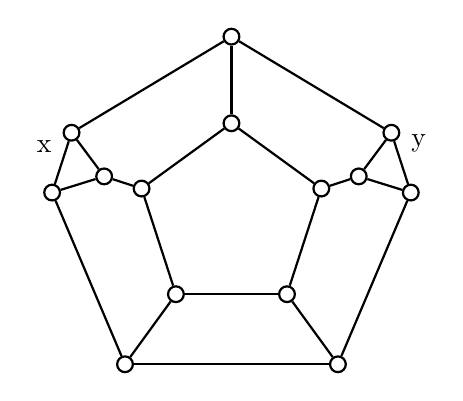
\begin{tikzpicture}[auto,
      specification/.style ={circle, draw, thick, inner sep = 0pt, minimum size=2mm}]
   \node[specification] (A1)  at (8:2.3cm)  {};
   
   \node[specification] (A)  at (18:1.7cm)  {};
   \node[specification] (A2)  at (28:2.3cm)  {};

   \node[specification] (B)  at (90:2.3cm)  {};
   \node[specification] (C1)  at (152:2.3cm)  {};   
   \node[specification] (C)  at (162:1.7cm)  {};
   \node[specification] (C2)  at (172:2.3cm)  {};

   \node[specification] (D) at (234:2.3cm)  {};
   \node[specification] (E)  at (306:2.3cm)  {};
   \node[specification] (F)  at (18:1.2cm)  {};
   \node[specification] (G)  at (90:1.2cm)  {};
   \node[specification] (H)  at (162:1.2cm)  {};
   \node[specification] (I) at (234:1.2cm)  {};
   \node[specification] (J) at (306:1.2cm)  {};


   \draw[thick] (A) to  (A1);
   \draw[thick] (A) to  (A2);
   \draw[thick] (A1) to node[swap] {y}  (A2);   
   \draw[thick] (A2) to  (B);
   \draw[thick] (B) to  (C1);

   \draw[thick] (C) to  (C1);
   \draw[thick] (C) to  (C2);
   \draw[thick] (C1) to node[swap] {x} (C2);
   \draw[thick] (C2) to  (D);
   \draw[thick] (D) to  (E);
   \draw[thick] (E) to  (A1);
   \draw[thick] (F) to  (G);
   \draw[thick] (G) to  (H);
   \draw[thick] (H) to  (I);
   \draw[thick] (I) to  (J);
   \draw[thick] (J) to  (F);

   \draw[thick] (A) to  (F);
   \draw[thick] (B) to  (G);
   \draw[thick] (C) to  (H);
   \draw[thick] (D) to  (I);
   \draw[thick] (E) to  (J);
 \end{tikzpicture}
\end{frame}

\begin{frame}
  \frametitle{9.2 非哈密顿平面图}
  \centering
      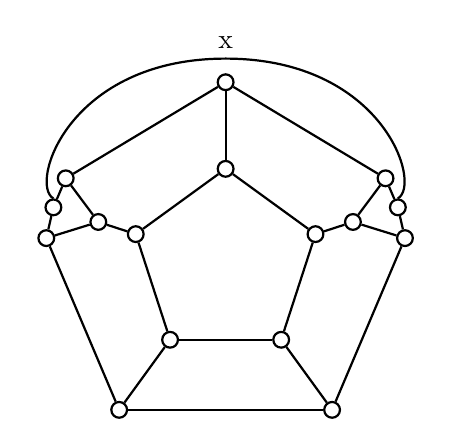
\begin{tikzpicture}[auto,
      specification/.style ={circle, draw, thick, inner sep = 0pt, minimum size=2mm}]
   \node[specification] (A1)  at (8:2.3cm)  {};
   \node[specification] (A3)  at (18:2.3cm)  {};   
   \node[specification] (A)  at (18:1.7cm)  {};
   \node[specification] (A2)  at (28:2.3cm)  {};

   \node[specification] (B)  at (90:2.3cm)  {};
   \node[specification] (C1)  at (152:2.3cm)  {};
   \node[specification] (C3)  at (162:2.3cm)  {};

   \node[specification] (C)  at (162:1.7cm)  {};
   \node[specification] (C2)  at (172:2.3cm)  {};

   \node[specification] (D) at (234:2.3cm)  {};
   \node[specification] (E)  at (306:2.3cm)  {};
   \node[specification] (F)  at (18:1.2cm)  {};
   \node[specification] (G)  at (90:1.2cm)  {};
   \node[specification] (H)  at (162:1.2cm)  {};
   \node[specification] (I) at (234:1.2cm)  {};
   \node[specification] (J) at (306:1.2cm)  {};


   \draw[thick] (A) to  (A1);
   \draw[thick] (A) to  (A2);
   \draw[thick] (A1) to   (A3);
   \draw[thick] (A3) to   (A2);

   \draw[thick] (A2) to  (B);
   \draw[thick] (B) to  (C1);

   \draw[thick] (C) to  (C1);
   \draw[thick] (C) to  (C2);
   \draw[thick] (C1) to  (C3);
   \draw[thick] (C3) to  (C2);
   \draw[thick] (C2) to  (D);
   \draw[thick] (D) to  (E);
   \draw[thick] (E) to  (A1);
   \draw[thick] (F) to  (G);
   \draw[thick] (G) to  (H);
   \draw[thick] (H) to  (I);
   \draw[thick] (I) to  (J);
   \draw[thick] (J) to  (F);

   \draw[thick] (A) to  (F);
   \draw[thick] (B) to  (G);
   \draw[thick] (C) to  (H);
   \draw[thick] (D) to  (I);
   \draw[thick] (E) to  (J);

   \draw[thick] (C3.north) .. controls  (-2.5cm, 1cm) and (-2.0cm, 2.6cm) .. (0cm,2.6cm) ..  controls (2.0cm, 2.6cm) and (2.5cm, 1cm)  ..  (A3.north);

   \node at (0cm, 2.8cm) {x};
   
 \end{tikzpicture}
\end{frame}

\begin{frame}
  \frametitle{9.2 非哈密顿平面图}
  \centering
  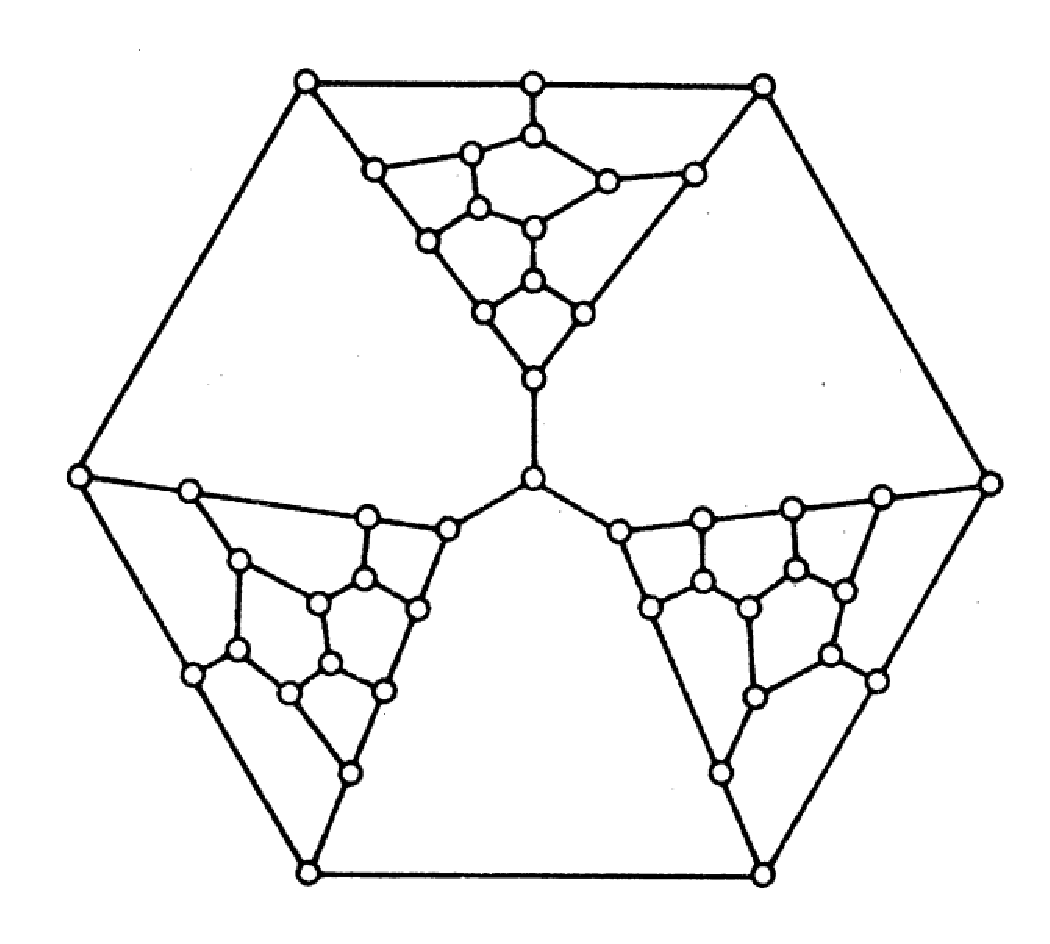
\includegraphics[width=7cm, height=6cm]{e4}
\end{frame}



\begin{frame}
  \frametitle{9.3 库拉托斯基定理、对偶图}
  \begin{definition9.3.1}
    设$x=uv$是图$G=(V,E)$的一条边,又$w$不是$G$的顶点,则当用边$uw$和$wv$代替边$x$时,就称$x$被细分。如果$G$的某些条边被细分,产生的图称为$G$的细分图。
  \end{definition9.3.1}
  \begin{definition9.3.2}
    两个图称为同胚的,如果它们都可以从同一个图通过一系列的边细分得到。
  \end{definition9.3.2}
  \begin{theorem9.3.1}
    一个图是可平面的充分必要条件是它没有同胚于$K_5$或$K_{3,3}$的子图。
  \end{theorem9.3.1}
\end{frame}
\begin{frame}
  \frametitle{9.3 库拉托斯基定理、对偶图}
  \begin{definition9.3.3}
    一个图$G$的一个初等收缩由等同两个临接的顶点$u$和$v$得到,即从$G$中
    去掉$u$和$v$,然后再加上一个新顶点$w$,使得$w$临接于所有临接
    于$u$或$v$的顶点。一个图$G$可以收缩到图$H$,如果$H$可以从$G$经过一系列的初等收缩得到。
  \end{definition9.3.3}
  \begin{theorem9.3.2}
    一个图是可平面的当且仅当它没有一个可以收缩到$K_5$或$K_{3,3}$的子图。
  \end{theorem9.3.2}
\end{frame}
\begin{frame}
  \frametitle{9.3 库拉托斯基定理、对偶图}
  \begin{definition9.3.4}
    设$G=(V,E)$是一个平面图,由$G$按照如下方法构造一个图$G^*$,$G^*$称为$G$的对偶图:对$G$的每个面$f$对应地有$G^*$的一个顶点$f^*$;对$G$的每条边$e$对应地有$G^*$的一条边$e^*$:$G^*$的两个顶点$f^*$与$g^*$由边$e^*$联结,当且仅当$G$中与顶点$f^*$与$g^*$对应的面$f$与$g$有公共边$e$,如果某条边$x$仅在一个面中出现而不是两个面的公共边,则在$G^*$中这个面对应的顶点有一个环。
  \end{definition9.3.4}
\end{frame}

\begin{frame}
  \frametitle{9.4 图的顶点着色}
  \begin{itemize}
  \item A fights with B and E;
  \item B fights with A and C;
  \item C fights with B, E and F;
  \item D fights with E;
  \item E fights with A, C and D;
    \item F fights with C.
  \end{itemize}
\end{frame}
\begin{frame}
  \frametitle{9.4 图的顶点着色}
  \begin{definition9.4.1}
    图的一种\alert{着色}是指对图的每个顶点指定一种颜色,使得没有两个临接的顶点有同一种颜色。图$G$的一个\alert{$n-$着色}是用$n$种颜色对$G$的着色。
  \end{definition9.4.1}
  \begin{definition9.4.2}
    图$G$的\alert{色数}是使$G$为$n-$着色的数$n$的最小值,图$G$的色数记为$\chi(G)$。若$\chi (G) \leq n$,则称$G$是\alert{$n-$可着色}的。若$\chi (G) = n$,则称$G$是\alert{$n$色}的。
  \end{definition9.4.2}
\end{frame}
\begin{frame}
  \frametitle{9.4 图的顶点着色}
  \begin{theorem9.4.1}
    一个图是可双色的当且仅当它没有奇数长的圈。
  \end{theorem9.4.1}
\vspace{1cm}
  \begin{minipage}{0.45\linewidth}
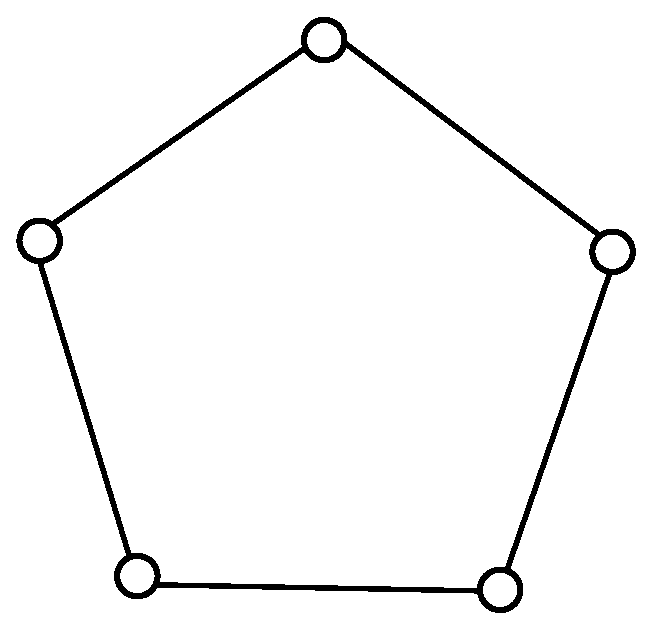
\includegraphics[width=4cm,height=3cm]{pentagon}    
  \end{minipage}
  \begin{minipage}{0.45\linewidth}
   
  \end{minipage}
\end{frame}

\begin{frame}
  \frametitle{9.4 图的顶点着色}
  \begin{theorem9.4.1}
    一个图是可双色的当且仅当它没有奇数长的圈。
  \end{theorem9.4.1}
\vspace{1cm}
  \begin{minipage}{0.45\linewidth}
\includegraphics[width=4cm,height=3cm]{pentagon1}    
  \end{minipage}
  \begin{minipage}{0.45\linewidth}
   
  \end{minipage}
\end{frame}
\begin{frame}
  \frametitle{9.4 图的顶点着色}
  \begin{theorem9.4.1}
    一个图是可双色的当且仅当它没有奇数长的圈。
  \end{theorem9.4.1}
\vspace{1cm}
  \begin{minipage}{0.45\linewidth}
\includegraphics[width=4cm,height=3cm]{pentagon2}    
  \end{minipage}
  \begin{minipage}{0.45\linewidth}
   
  \end{minipage}
\end{frame}

\begin{frame}
  \frametitle{9.4 图的顶点着色}
  \begin{theorem9.4.1}
    一个图是可双色的当且仅当它没有奇数长的圈。
  \end{theorem9.4.1}
\vspace{1cm}
  \begin{minipage}{0.45\linewidth}
\includegraphics[width=4cm,height=3cm]{pentagon3}    
  \end{minipage}
  \begin{minipage}{0.45\linewidth}
   
  \end{minipage}
\end{frame}
\begin{frame}
  \frametitle{9.4 图的顶点着色}
  \begin{theorem9.4.1}
    一个图是可双色的当且仅当它没有奇数长的圈。
  \end{theorem9.4.1}
\vspace{1cm}
  \begin{minipage}{0.45\linewidth}
\includegraphics[width=4cm,height=3cm]{pentagon4}    
  \end{minipage}
  \begin{minipage}{0.45\linewidth}
   
  \end{minipage}
\end{frame}
\begin{frame}
  \frametitle{9.4 图的顶点着色}
  \begin{theorem9.4.1}
    一个图是可双色的当且仅当它没有奇数长的圈。
  \end{theorem9.4.1}
\vspace{1cm}
  \begin{minipage}{0.45\linewidth}
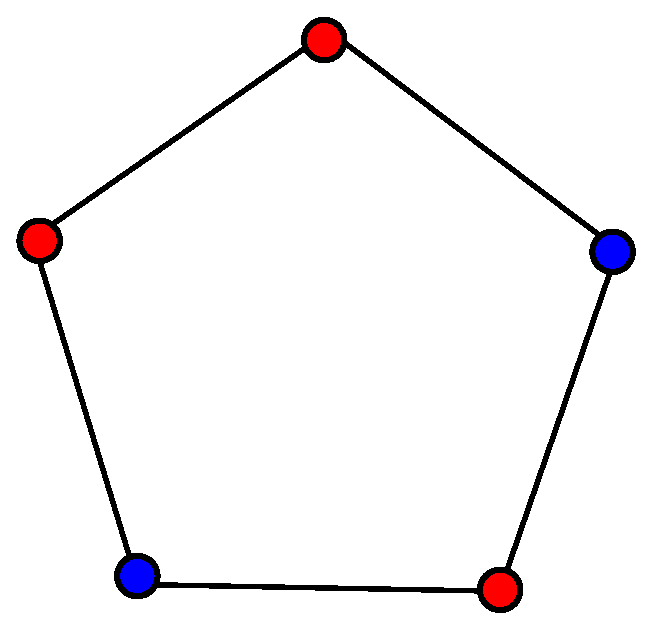
\includegraphics[width=4cm,height=3cm]{pentagon5}    
  \end{minipage}
  \begin{minipage}{0.45\linewidth}
   
  \end{minipage}
\end{frame}

\begin{frame}
  \frametitle{9.4 图的顶点着色}
  \begin{theorem9.4.1}
    一个图是可双色的当且仅当它没有奇数长的圈。
  \end{theorem9.4.1}
\vspace{1cm}
  \begin{minipage}{0.45\linewidth}
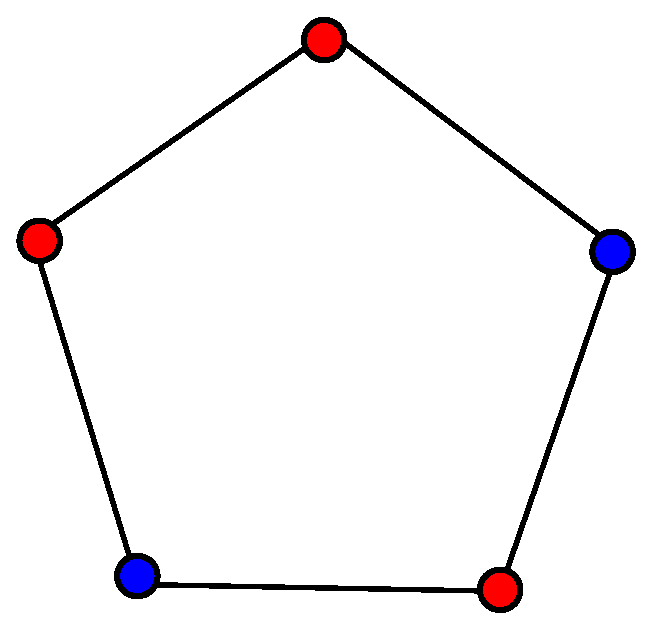
\includegraphics[width=4cm,height=3cm]{pentagon5}    
  \end{minipage}
  \begin{minipage}{0.45\linewidth}
    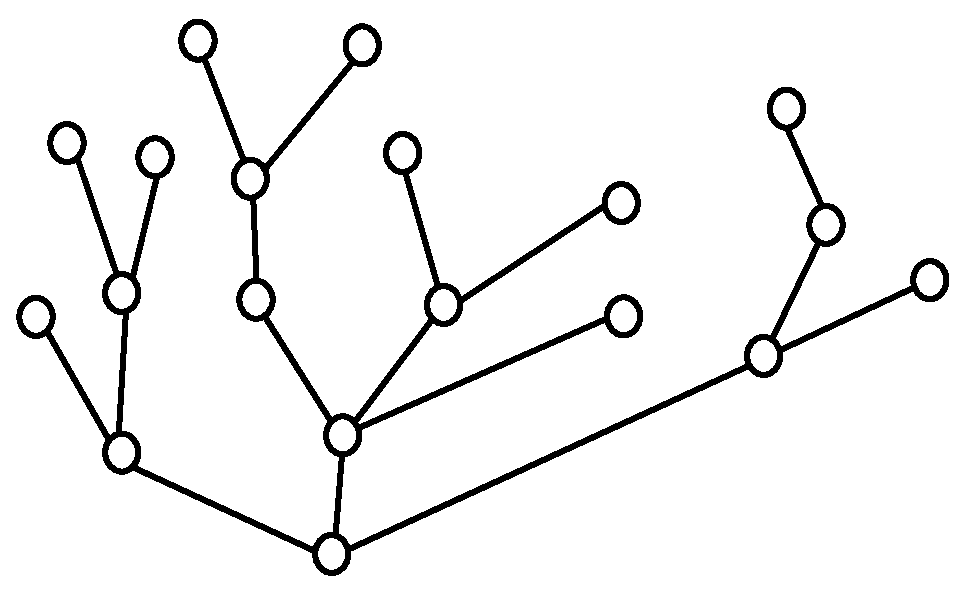
\includegraphics[width=4cm,height=3cm]{color2}
  \end{minipage}
\end{frame}
\begin{frame}
  \frametitle{9.4 图的顶点着色}
  \begin{theorem9.4.1}
    一个图是可双色的当且仅当它没有奇数长的圈。
  \end{theorem9.4.1}
\vspace{1cm}
  \begin{minipage}{0.45\linewidth}
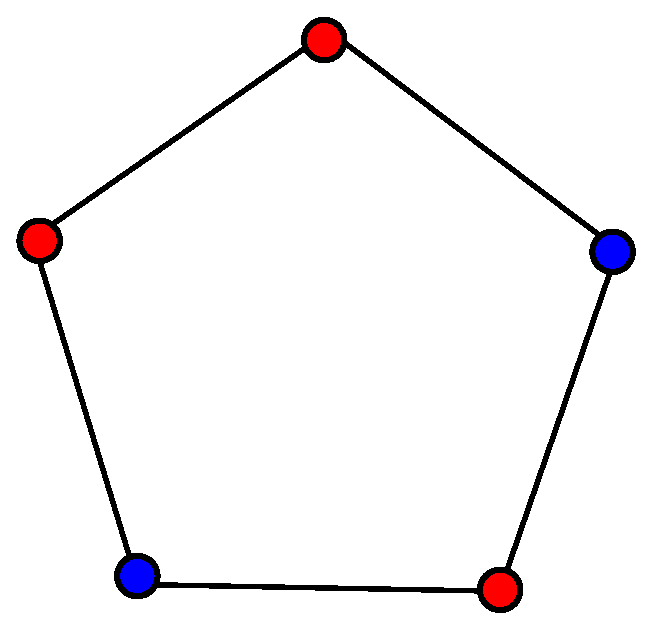
\includegraphics[width=4cm,height=3cm]{pentagon5}    
  \end{minipage}
  \begin{minipage}{0.45\linewidth}
    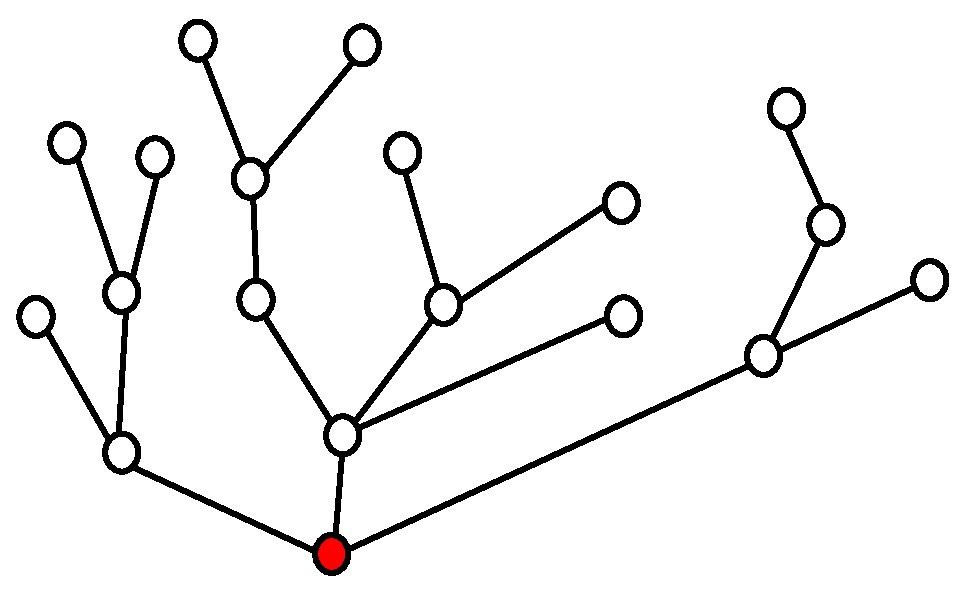
\includegraphics[width=4cm,height=3cm]{color21}
  \end{minipage}
\end{frame}

\begin{frame}
  \frametitle{9.4 图的顶点着色}
  \begin{theorem9.4.1}
    一个图是可双色的当且仅当它没有奇数长的圈。
  \end{theorem9.4.1}
\vspace{1cm}
  \begin{minipage}{0.45\linewidth}
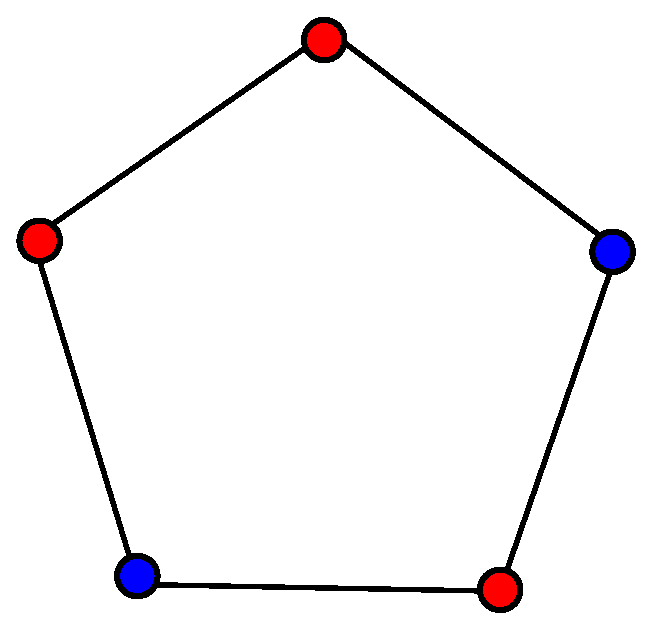
\includegraphics[width=4cm,height=3cm]{pentagon5}    
  \end{minipage}
  \begin{minipage}{0.45\linewidth}
    \includegraphics[width=4cm,height=3cm]{color22}
  \end{minipage}
\end{frame}
\begin{frame}
  \frametitle{9.4 图的顶点着色}
  \begin{theorem9.4.1}
    一个图是可双色的当且仅当它没有奇数长的圈。
  \end{theorem9.4.1}
\vspace{1cm}
  \begin{minipage}{0.45\linewidth}
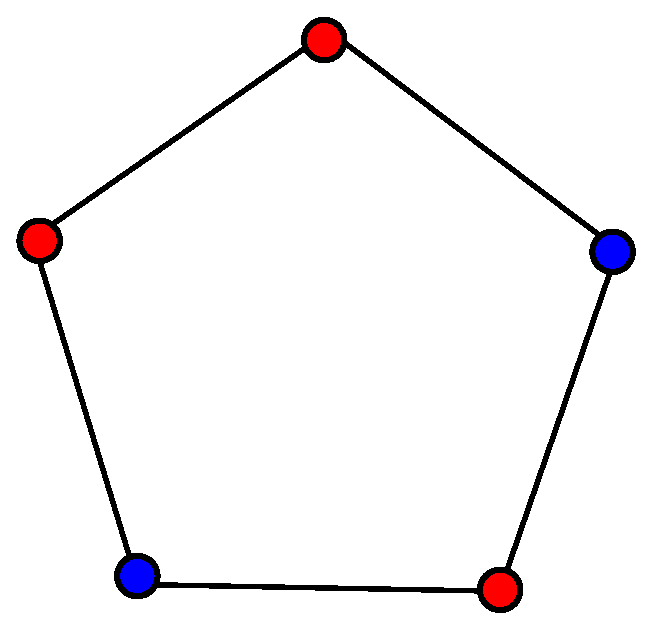
\includegraphics[width=4cm,height=3cm]{pentagon5}    
  \end{minipage}
  \begin{minipage}{0.45\linewidth}
    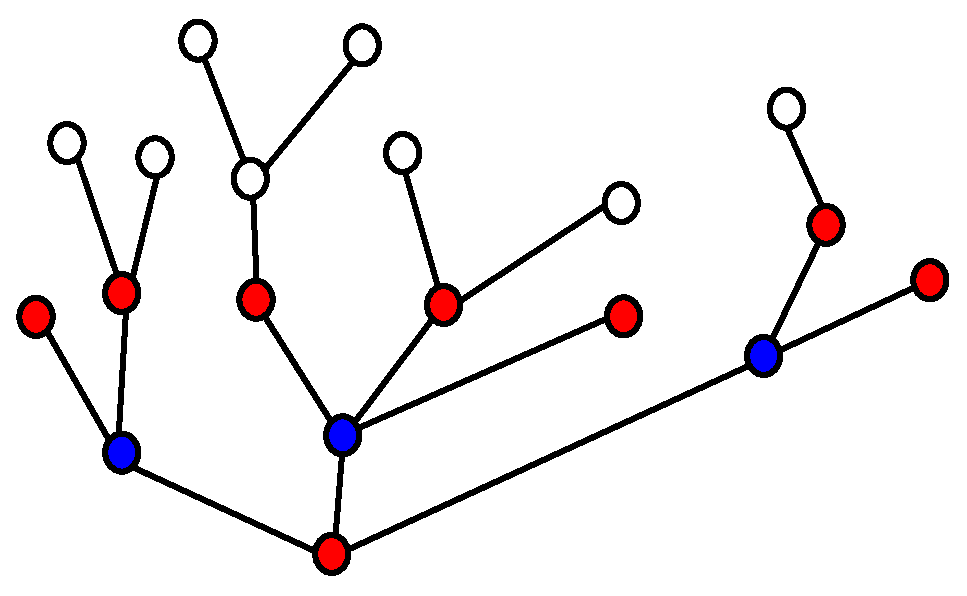
\includegraphics[width=4cm,height=3cm]{color23}
  \end{minipage}
\end{frame}
\begin{frame}
  \frametitle{9.4 图的顶点着色}
  \begin{theorem9.4.1}
    一个图是可双色的当且仅当它没有奇数长的圈。
  \end{theorem9.4.1}
\vspace{1cm}
  \begin{minipage}{0.45\linewidth}
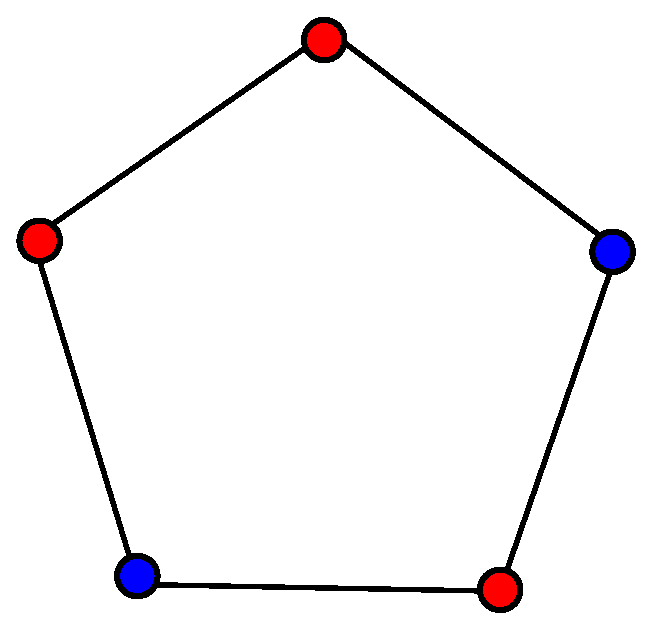
\includegraphics[width=4cm,height=3cm]{pentagon5}    
  \end{minipage}
  \begin{minipage}{0.45\linewidth}
    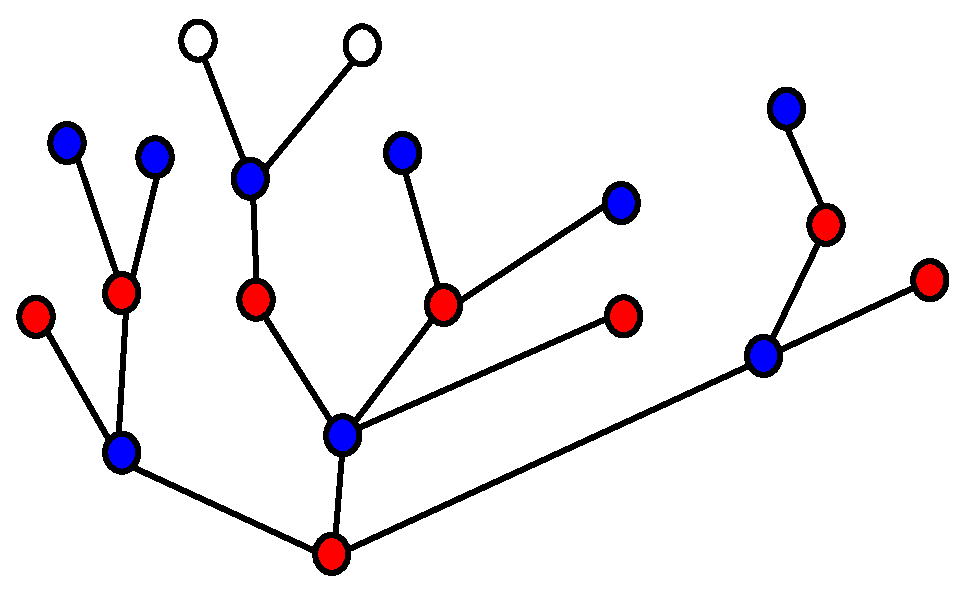
\includegraphics[width=4cm,height=3cm]{color24}
  \end{minipage}
\end{frame}
\begin{frame}
  \frametitle{9.4 图的顶点着色}
  \begin{theorem9.4.1}
    一个图是可双色的当且仅当它没有奇数长的圈。
  \end{theorem9.4.1}
\vspace{1cm}
  \begin{minipage}{0.45\linewidth}
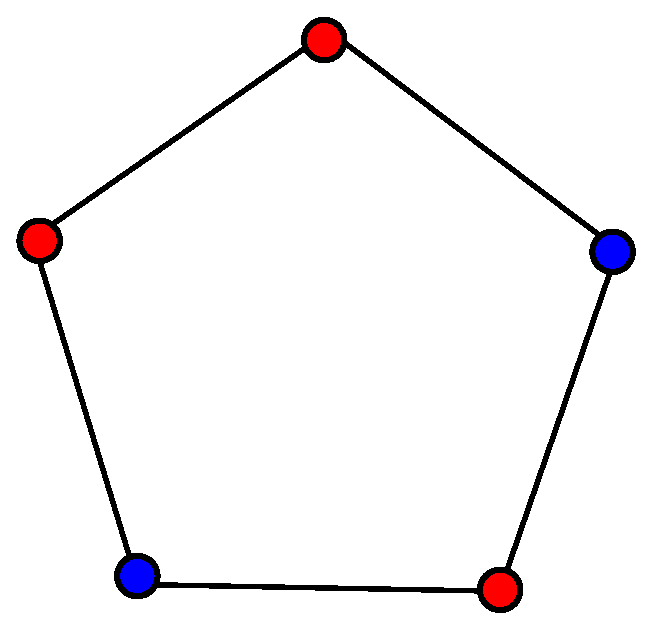
\includegraphics[width=4cm,height=3cm]{pentagon5}    
  \end{minipage}
  \begin{minipage}{0.45\linewidth}
    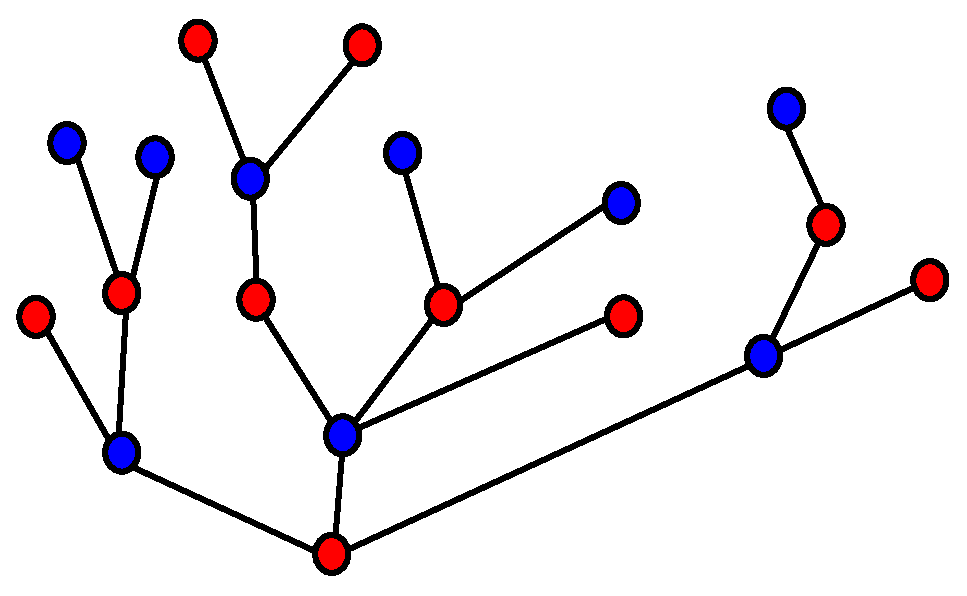
\includegraphics[width=4cm,height=3cm]{color25}
  \end{minipage}
\end{frame}

\begin{frame}
  \frametitle{9.4 图的顶点着色}
  \begin{theorem9.4.1}
    一个图是可双色的当且仅当它没有奇数长的圈。
  \end{theorem9.4.1}
\vspace{1cm}
  \begin{minipage}{0.45\linewidth}
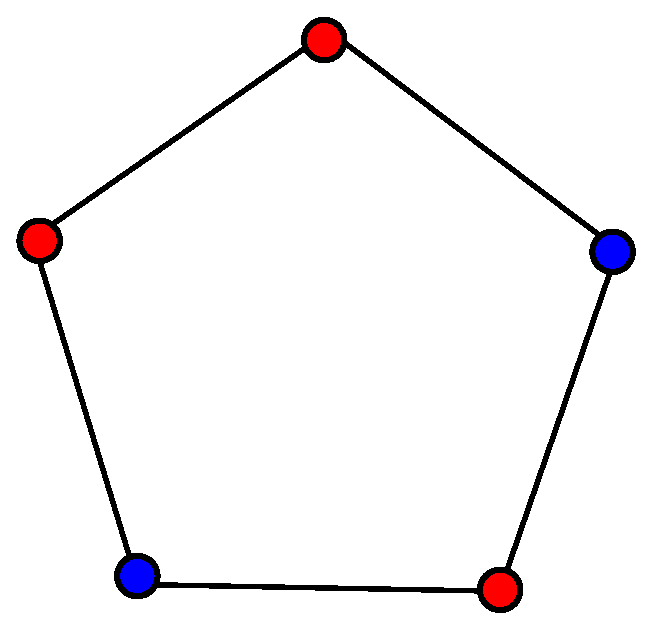
\includegraphics[width=4cm,height=3cm]{pentagon5}    
  \end{minipage}
  \begin{minipage}{0.45\linewidth}
    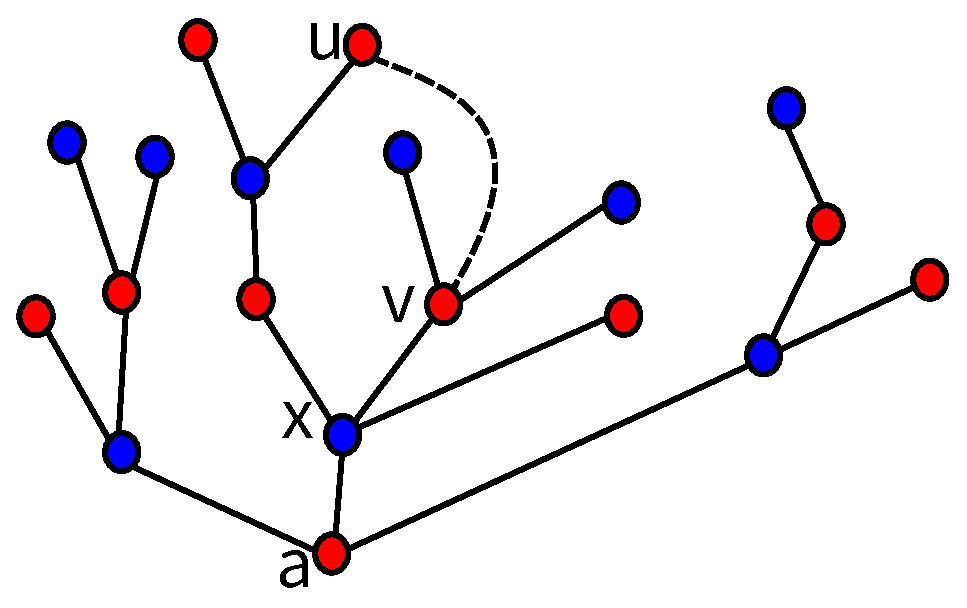
\includegraphics[width=4cm,height=3cm]{color26}
  \end{minipage}
\end{frame}

\begin{frame}
  \frametitle{9.4 图的顶点着色}
  \begin{theorem9.4.1}
    一个图是可双色的当且仅当它没有奇数长的圈。
  \end{theorem9.4.1}
  \begin{proof}[证明]
    设图$G$为可双色的,则显然图$G$没有奇数长的圈。这是因为假设图$G$有奇数长的圈$C$,
  则$C$是3色的,从而$\chi(G) \geq 3$,与$G$是可双色的矛盾。  
  \end{proof}
\end{frame}

\begin{frame}
  \frametitle{9.4 图的顶点着色}
  \begin{theorem9.4.1}
    一个图是可双色的当且仅当它没有奇数长的圈。
  \end{theorem9.4.1}
  \begin{proof}[证明(续上页)]
   

  设图$G$没有奇数长的圈,以下给出一种用两种颜色对$G$的顶点进行着色的算法,从而证明图$G$是可双色的。不妨设图$G$是连通的,否则可以对图$G$的每个连通分量分别进行着色。任取$G$的一个顶点$a$,对其着红色,然后对与顶点$a$邻接的顶点着蓝色,接下来对所有与已经着色的顶点相邻接的顶点着红色,这样依次下去,每次都对所有与已经着色的顶点相邻接的顶点着与前一次的着色不同的另一种颜色。该算法结束时用至多两种颜色对$G$的顶点进行了着色。
  
  \end{proof}
\end{frame}
\begin{frame}
  \frametitle{9.4 图的顶点着色}
  \begin{theorem9.4.1}
    一个图是可双色的当且仅当它没有奇数长的圈。
  \end{theorem9.4.1}
  \begin{proof}[证明(续上页)]
    以下证明每次对所有与已经着色的顶点相邻接的顶点着与前一次的着色不同的另一种颜色时,
不会产生相邻的两个顶点着以相同颜色的情况,从而保证前面的算法是正确的。用反证法。
假设对顶点$u$进行着色时,不妨设对其着红色,已经有一个与之相邻的顶点$v$着了红色。
从着色的过程知,从顶点$a$到顶点$u$之间有一条路$P_1$,其上的顶点依次着了红色和蓝色,
从顶点$a$到顶点$v$之间也有一条路$P_2$,其上的顶点依次着了红色和蓝色。
取$P_1$和$P_2$的最后一个公共的顶点$x$,则$P_1$上从顶点$u$到顶点$x$的路与$P_2$上从顶点$x$到顶点$v$的路和边$vu$一起构成一个圈,该圈上$u$和$v$着相同的颜色,其他各顶点依次着不同的颜色,因此其长度为奇数,与$G$中没有奇数长的圈矛盾。 
  \end{proof}
\end{frame}

\begin{frame}
  \frametitle{9.4 图的顶点着色}
  \begin{theorem9.4.2}
    设$\Delta = \Delta (G)$为图$G$的顶点度的最大值,则$G$是$(\Delta+1)-$可着色的。
  \end{theorem9.4.2}
\end{frame}
\begin{frame}
  \frametitle{9.4 图的顶点着色}
  \begin{theorem9.4.3}
    如果$G$是一个连通图且不是完全图也不是奇数长的圈,则$G$是$\Delta(G)-$可着色的。
  \end{theorem9.4.3}
\end{frame}
\begin{frame}
  \frametitle{9.4 图的顶点着色}
  \begin{theorem9.4.4}
    每个平面图是$6-$可着色的。
  \end{theorem9.4.4}
\end{frame}
\begin{frame}
  \frametitle{9.4 图的顶点着色}
  \begin{theorem9.4.5}
    每个平面图是$5-$可着色的。
  \end{theorem9.4.5}
\vspace{1cm}
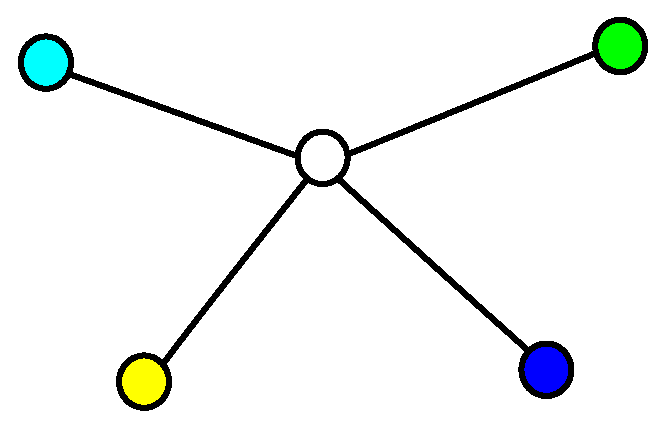
\includegraphics[width=4cm,height=3cm]{color52}
\end{frame}
\begin{frame}
  \frametitle{9.4 图的顶点着色}
  \begin{theorem9.4.5}
    每个平面图是$5-$可着色的。
  \end{theorem9.4.5}
\vspace{1cm}
\includegraphics[width=4cm,height=3cm]{color53}
\end{frame}

\begin{frame}
  \frametitle{9.4 图的顶点着色}
  \begin{theorem9.4.5}
    每个平面图是$5-$可着色的。
  \end{theorem9.4.5}
\vspace{1cm}
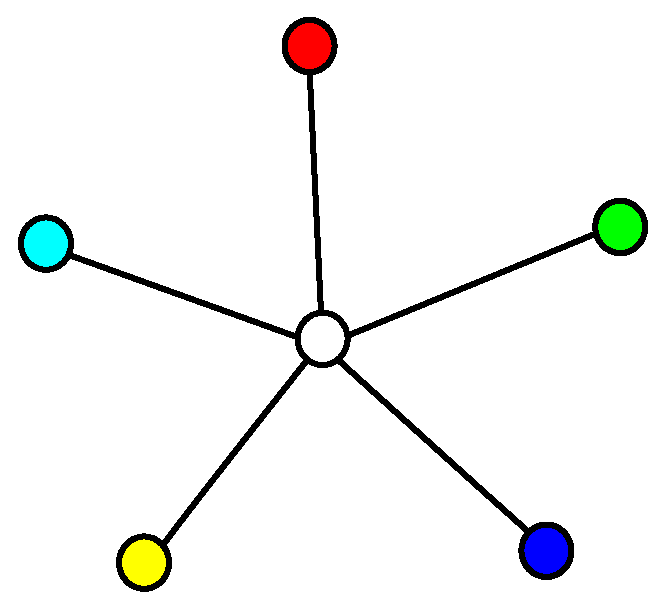
\includegraphics[width=4cm,height=3cm]{color51}
\end{frame}

\begin{frame}
  \frametitle{9.4 图的顶点着色}
  \begin{theorem9.4.6}
    每个平面图是$4-$可着色的。
  \end{theorem9.4.6}
\end{frame}
\begin{frame}
  \frametitle{习题}
  \begin{Exercise}
    证明:若$G$的任两个奇数长的圈都有一个公共顶点,则$\chi(G)\leq 5$。
  \end{Exercise}
\end{frame}
\end{CJK}
\end{document}

%%% Local Variables:
%%% mode: latex
%%% TeX-master: t
%%% End:
